\lstinputlisting[language=bash,basicstyle=\small]{python_codes/fieldstone_78/keywords}

\begin{center}
Code at \url{https://github.com/cedrict/fieldstone/tree/master/python_codes/fieldstone_78}
\end{center}

\par\noindent\rule{\textwidth}{0.4pt}

%%%%%%%%%%%%%%%%%%%%%%%%%%%%%%%%%%%%%%%%%%%%%%%%%%%%%%%%%%%%%%%%%%%%%%%%%%%%%%%%%%%%%%%%%%%%%%%%%%%%


Although the $Q_1\times P_0$ is not LBB-stable (see Section~\ref{ss:LBBcond})
it has been proven that some spatial arrangements of this element can be, such as the
following macro-element:

\begin{center}
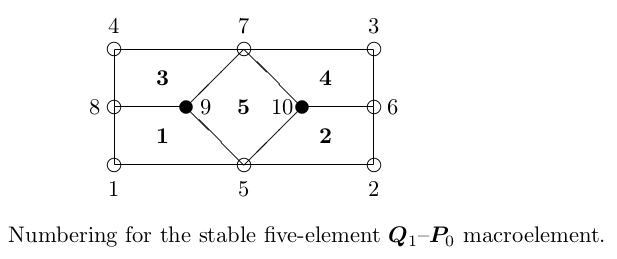
\includegraphics[width=5cm]{python_codes/fieldstone_78/images/elsw}
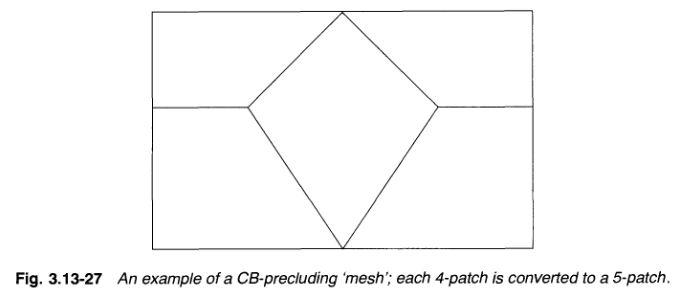
\includegraphics[width=5cm]{python_codes/fieldstone_78/images/grsa}\\
{\captionfont Left: Fig 3.12 of Elman et al book \cite{elsw}.
Right: Taken from Gresho \& Sani's book \cite{grsa}: "For fans of $Q_1Q_0$ who want 
guaranteed optimal convergence of both u and p (with however larger error 
constants caused by the distorted shapes?), one way to assure this is
to discretise via the macro elements above, each composed of five $Q_1Q_0$
quadrilaterals. Such checkerboard-killer meshes have been employed in practice
by (at least) Bath\'e \cite{chba93}. Both the macro-element and the proof are
due to Stenberg \cite{sten84}."}
\end{center}

\begin{center}
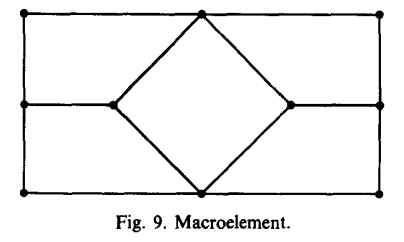
\includegraphics[width=5cm]{python_codes/fieldstone_78/images/chba93}\\
{\captionfont Taken from Chapelle \& Bathe \cite{chba93}: "the numerical inf-sup test is passed for this mesh and in fact,
this behavior was proven analytically (see Brezzi \& Fortin \cite{brfo}, see also Le Tallec \& Ruas \cite{leru86}).}
\end{center}

\begin{center}
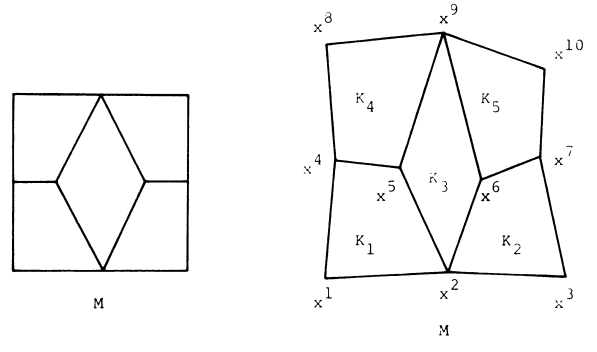
\includegraphics[width=5cm]{python_codes/fieldstone_78/images/sten84}
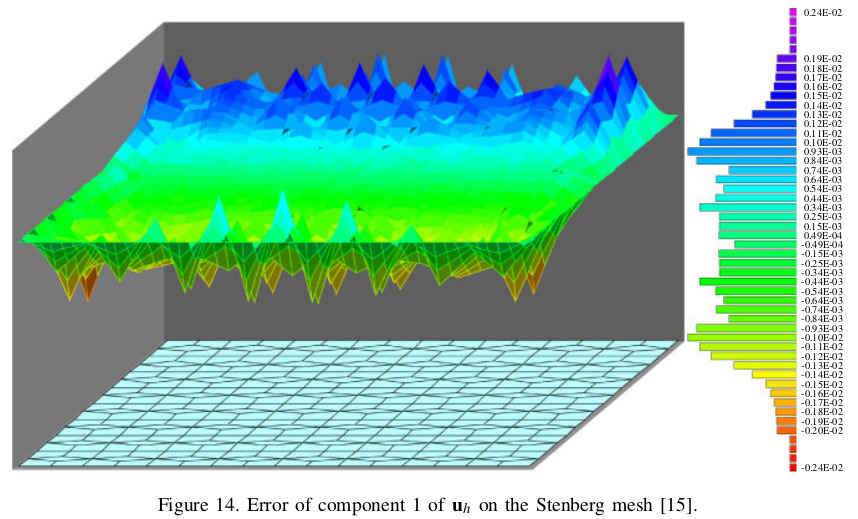
\includegraphics[width=5cm]{python_codes/fieldstone_78/images/qizh07}\\
{\captionfont Left: Taken from Stenberg (1984) \cite{sten84}. 
Right: Taken from Qin \& Zhang (2007) \cite{qizh07}.}
\end{center}

On the following a mesh is shown which consists of $16\times 16$ macroelements:

\begin{center}
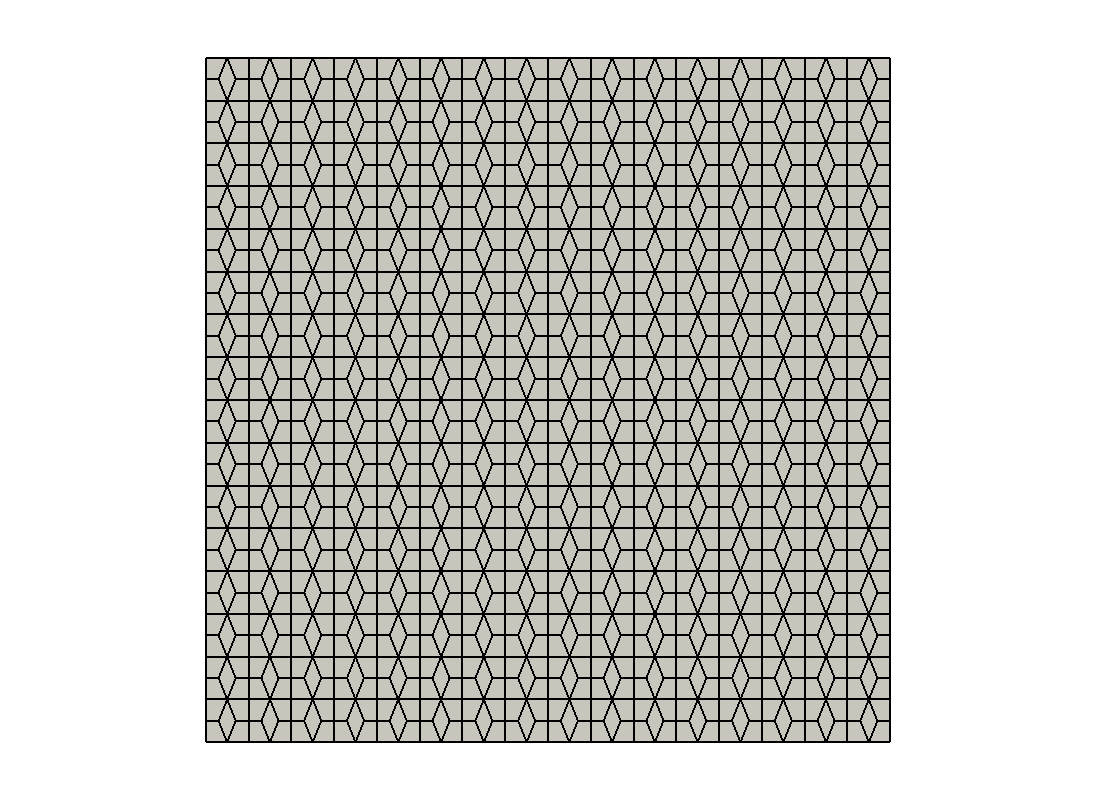
\includegraphics[width=8cm]{python_codes/fieldstone_78/images/mesh}\\
{\captionfont Mesh composed of 16x16 macroelements}
\end{center}
Note that in this implementation all 5 elements of the macro-element have the 
same area. 

Normalisation is achieved by setting $p=0$ on the last element and then 
renormalising the pressure field.

%...................
\paragraph{Results}

We start with the Donea \& Huerta manufactured solution (see Section~\ref{mms1}) and 
proceed to compute the velocity and pressure error convergence as a function of the 
element size which is take to be $h = \sqrt{L_xL_y/nel}$. We see that 
the errors converge as expected, quadratically for the velocity and linearly for the pressure:

\begin{center}
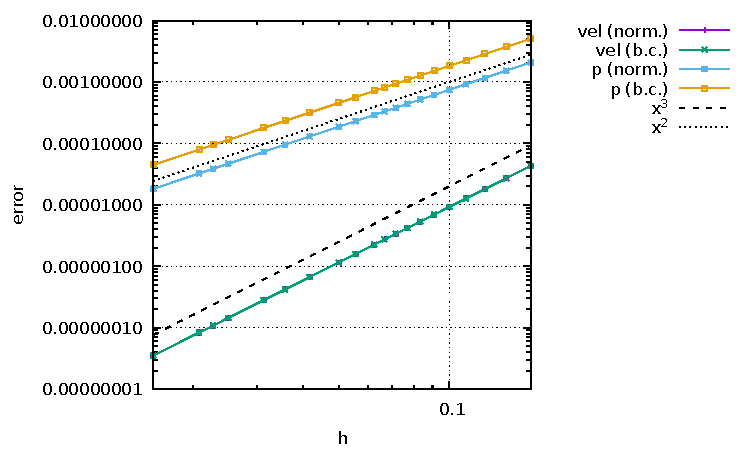
\includegraphics[width=7cm]{python_codes/fieldstone_78/results/errors.pdf}
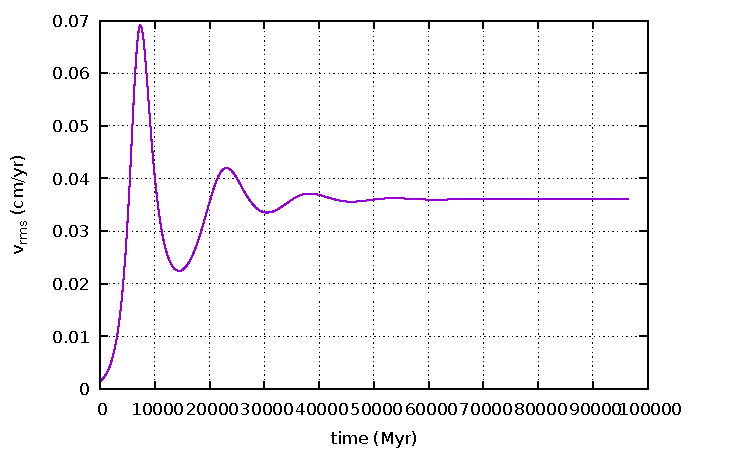
\includegraphics[width=7cm]{python_codes/fieldstone_78/results/vrms.pdf}
\end{center}

On the following figures the pressure is plotted agains the analytical solution and 
we see that there is no checkerboarding occurring:

\begin{center}
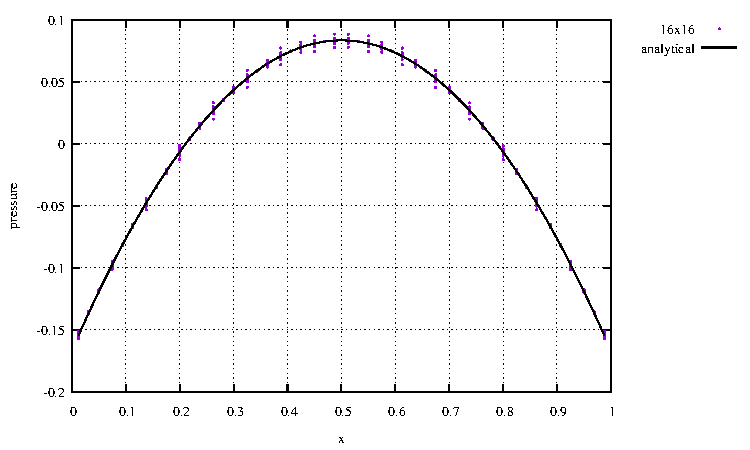
\includegraphics[width=7cm]{python_codes/fieldstone_78/results/pressure16}
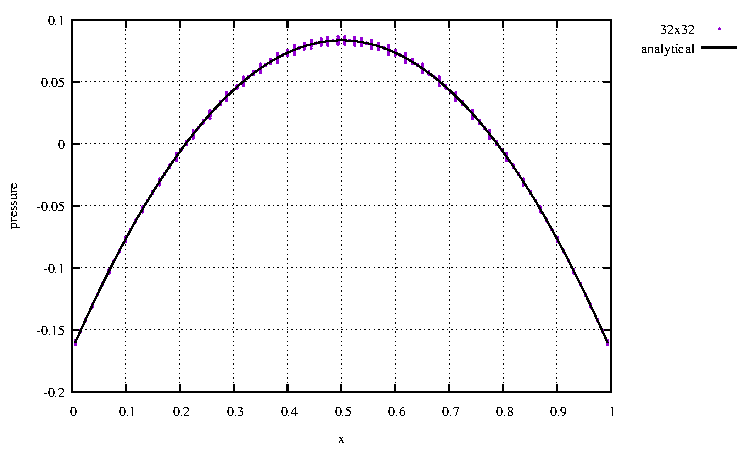
\includegraphics[width=7cm]{python_codes/fieldstone_78/results/pressure32} \\
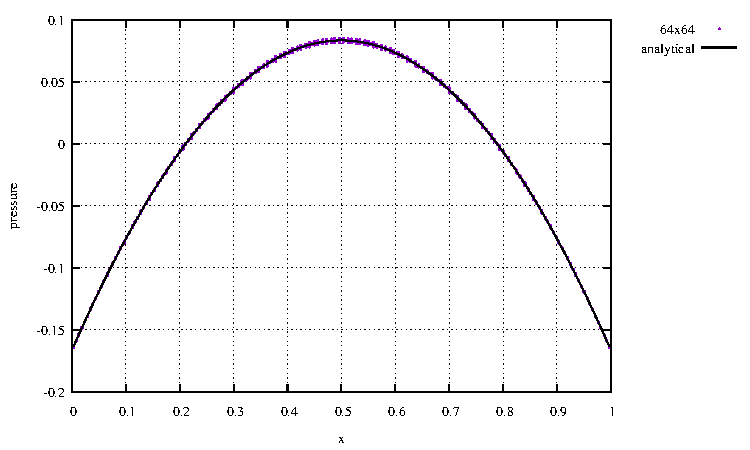
\includegraphics[width=7cm]{python_codes/fieldstone_78/results/pressure64}
\includegraphics[width=7cm]{python_codes/fieldstone_78/results/pressure96}
\end{center}

Rather interestingly the pressure error is the largest next to the boundaries:
\begin{center}
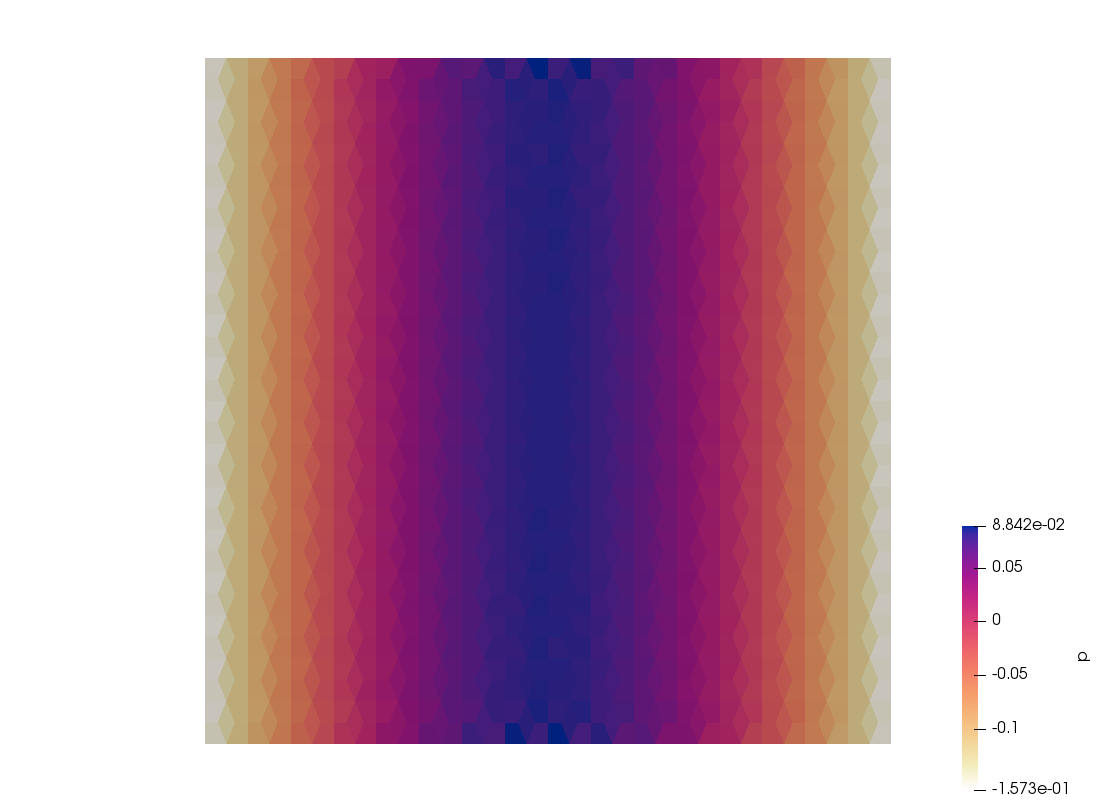
\includegraphics[width=7cm]{python_codes/fieldstone_78/results/p16x16}
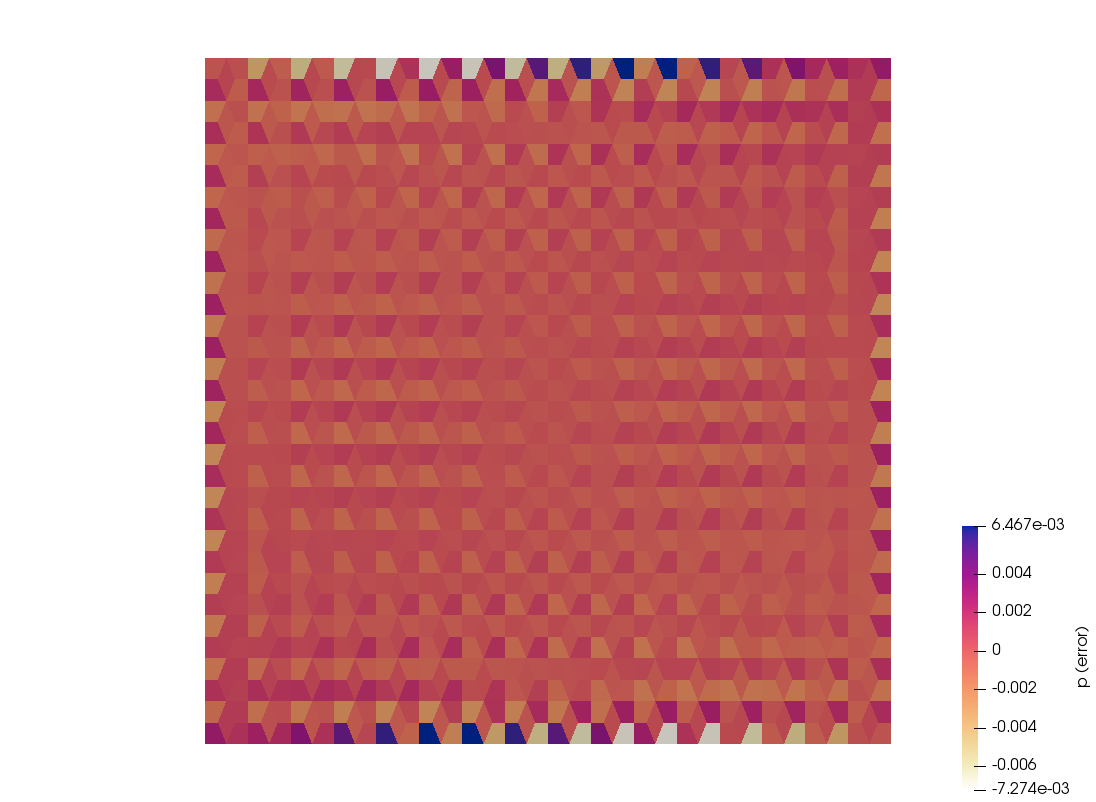
\includegraphics[width=7cm]{python_codes/fieldstone_78/results/p16x16_error}\\
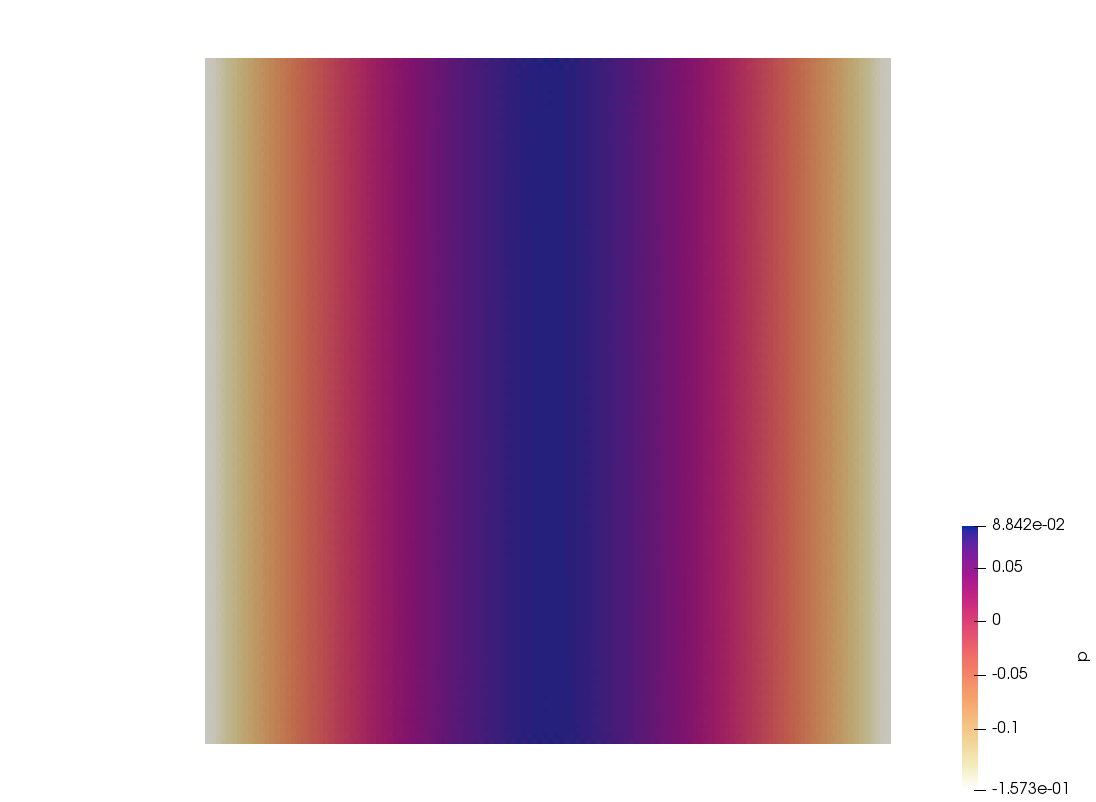
\includegraphics[width=7cm]{python_codes/fieldstone_78/results/p64x64}
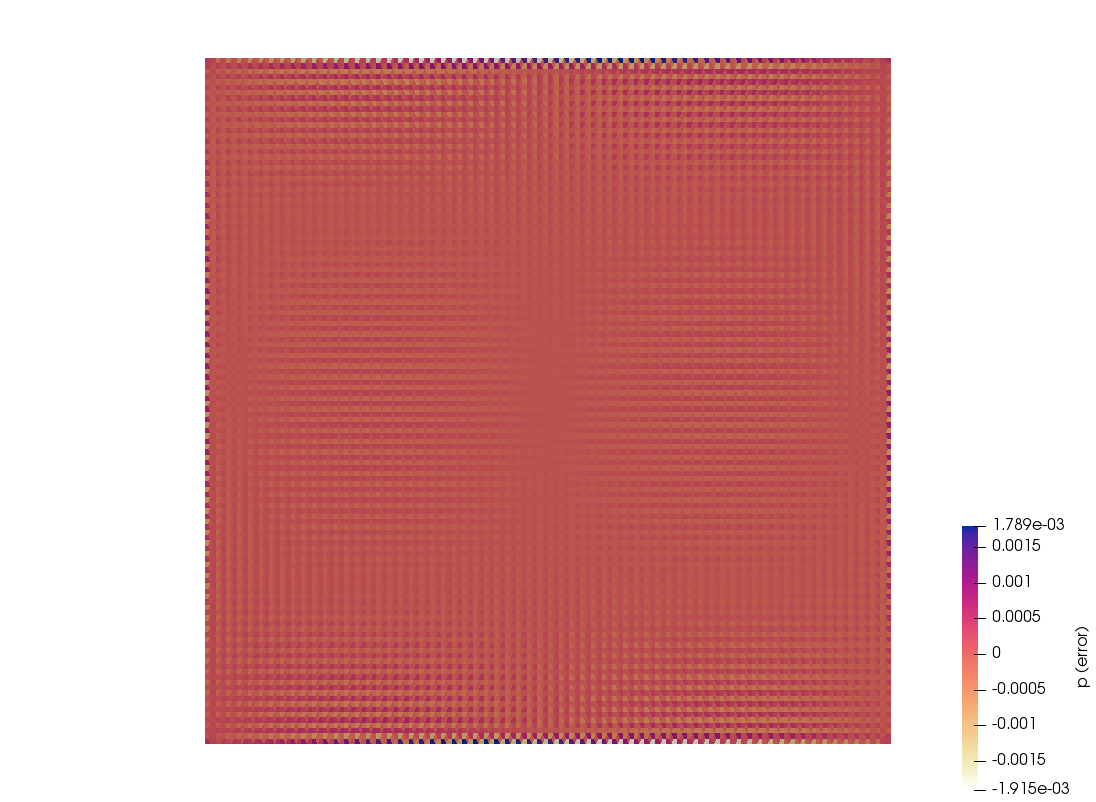
\includegraphics[width=7cm]{python_codes/fieldstone_78/results/p64x64_error}\\
{\captionfont Top row: 16x16 mesh, bottom row: 64x64 mesh}
\end{center}

Discussion

what is the real advantage of such a macro-element? it is LBB stable, so 
iterative solver will work optimally, and the pressure has no checkerboard. 
On the other hand it is anisotropic since the 'diamonds are vertical'. 
Also if one would consider a macro-element as an element, it counts 10 velocity nodes and 5 pressures, 
which makes it much more expensive than a $Q_2\times Q_1$ element of the same size...


